\chapter{Návrh syntetizátora}
\section{Návrh architektúry syntetizátora}

Prvým krokom návrhu syntetizátora by mal byť návrh jeho architektúry, popis komponentov a ich úloha v celom systéme. Na obrázku \ref{obr06a} je znázornený základný princíp fungovania s polyfonickými hlasmi.

\begin{figure}[h]
\centering
\resizebox{14cm}{!}{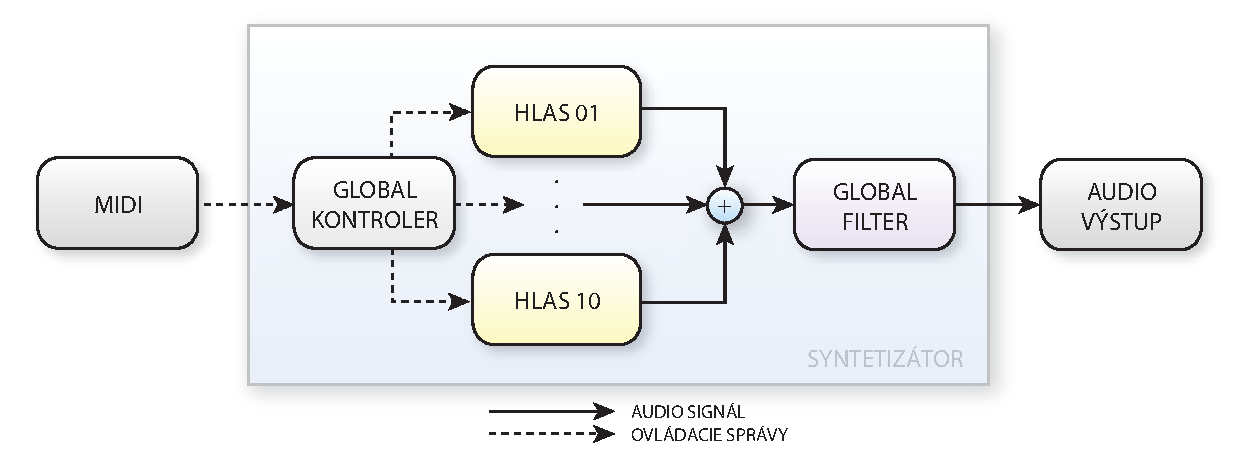
\includegraphics{d04a}}
\caption{\label{obr06a} Architektúra syntetizátora}
\end{figure}

Syntetizátor prijíma MIDI správy, GLOBAL KONTROLER ich analyzuje a relevantné správy posiela jednotlivým hlasom polyfónie. Syntetizátor disponuje polyfóniou 10 hlasov. Ich jednotlivé signály sa sčítavajú a vysledný signál sa filtruje v bloku GLOBAL FILTER od nepočuteľných nízkych frekvencií. Vyfiltrovaný signál sa posiela na výstup.

Obrázok \ref{obr06b} znázorňuje štruktúru jednotlivých polyfonických hlasov, bloky komponentov a toky signálov a správ medzi nimi. 

\begin{figure}[h]
\centering
\resizebox{!}{8cm}{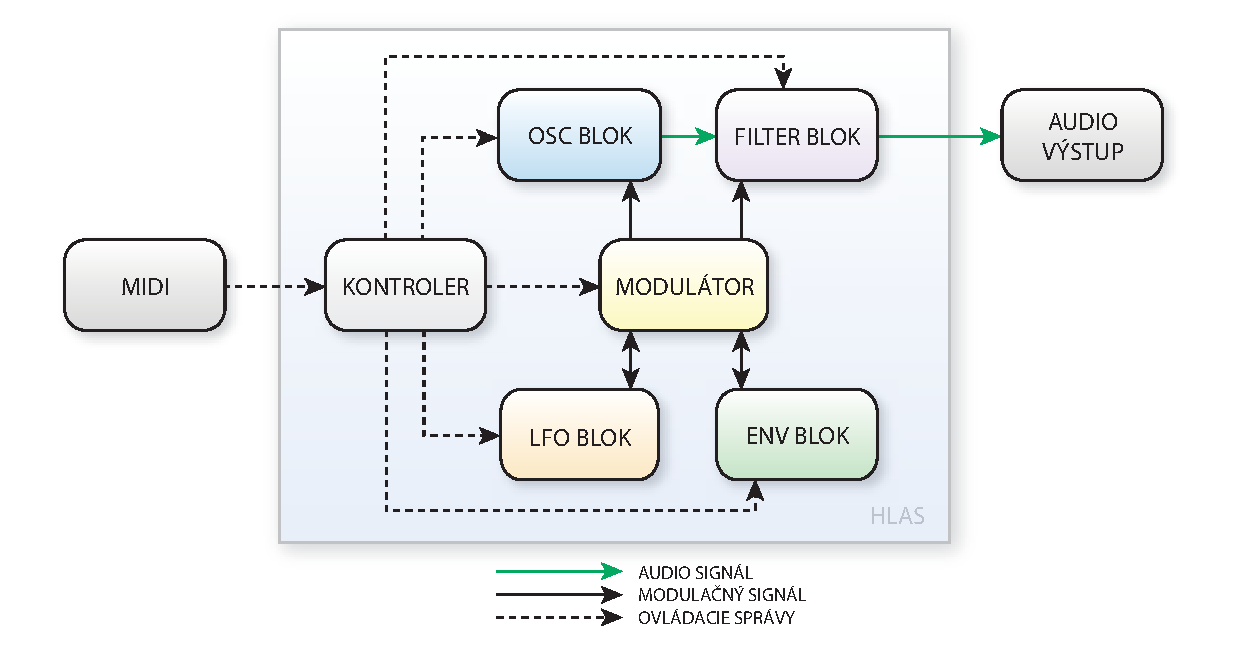
\includegraphics{d03a}}
\caption{\label{obr06b} Štruktúra hlasu polyfónie}
\end{figure}

Blok KONTROLER analyzuje prijaté MIDI správy a distribuuje ich ostatným blokom. Bloky OSC, LFO, ENV a FILTER prijímajú len MIDI noty, MODULÁTOR prijíma aj ostatné správy, ktoré syntetizátor podporuje. MODULÁTOR prijíma aj signály generované blokmi LFO a ENV a vysiela modulačné signály do všetkých štyroch funkčných blokov. Blok OSC je zodpovedný za generovanie zvukového signálu a blok filter filtruje tento signál. Zvukový výstup z filtra sa posiela na výstup celého hlasu.

\section{Funkčné bloky architektúry}

\subsubsection*{OSC blok}

OSC blok sa skladá zo štyroch oscilátorov, mixéra a zosilňovača. Oscilátory generujú jednoduchý signál, v mixéri sa sčítavajú, pričom amplitúdy a smerovania\newfootnote{Smerovanie (pan) v kontexte zvukového signálu je jeho pozícia medzi pravým a ľavým kanálom.} výstupov jednotlivých oscilátorov je možné ovládať parametrami a moduláciami. Signál z mixéra ešte prechádza zosilňovačom. Jeho úloha je dynamicky ovládať amplitúdu výstupu OSC bloku, najčastejšie podľa 
obálky.

\subsubsection*{FILTER blok}

FILTER blok filtruje signál dvoma filtrami, ktoré môžu byť zapojené sériovo alebo paralelne, a filtrovaný signál posiela na výstup.

\subsubsection*{LFO blok}

LFO blok obsahuje štyri nízkofrekvenčné oscilátory a nimi vygenerovaný signál posiela modulátoru.

\subsubsection*{ENV blok}

ENV blok obsahuje štyri generátory obálok a vygenerovaný signál posiela modulátoru.

\subsubsection*{MODULÁTOR}

MODULÁTOR je blok, ktorý obsahuje prostriedky na distribúciu modulačných signálov modulovaným parametrom podľa modulačnej matice. Modulačná matica je zoznam modulácií (trojíc - zdroj, cieľ a miera modulácie), podľa ktorej sa modulujú signály a parametre v syntetizátore.

\section{Návrh komponentov}
Základné funkcie jednotlivých komponentov už boli opísané. V tejto sekcii sa zameriam na vyšpecifikovanie požiadaviek na jednotlivé komponenty.

\subsection{Oscilátor}
\begin{figure}[h]
\centering
\resizebox{15cm}{!}{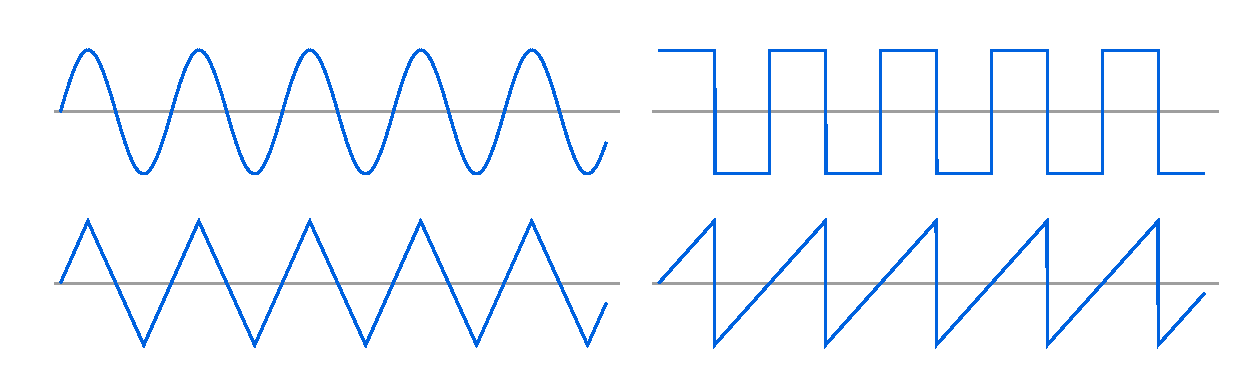
\includegraphics{waves}}
\caption{\label{obr12} Základné analógové priebehy}
\end{figure}

Oscilátor by mal disponovať piatimi základnými priebehmi:
\begin{itemize}
\setlength{\itemsep}{-0.5ex}
\item sínus,
\item píla,
\item trojuholník,
\item obdĺžnik,
\item šum.
\end{itemize}

Počítanie týchto priebehov by bolo zbytočne náročné na výkon procesora, a preto by mal syntetizátor tieto priebehy predpočítať v dostatočnom rozlíšení a uložiť do pamäte.

Priebehy \emph{píla}, \emph{trojuholník} a \emph{obdĺžnik} ale nie je také jednoduché vytvoriť, pretože jednoduchý geometricky presný priebeh nezodpovedá v navzorkovanom signále signálu analógovému. Pri jeho prehrávaní by vznikli digitálne artefakty vo forme nežiaducich frekvencií -- aliasy. Tu vzniká potreba návrhu nejakého antialiasového opatrenia. 

\subsubsection{Antialiasing oscilátora}
\label{antialiasing}
\begin{figure}[h]
\centering
\resizebox{15cm}{!}{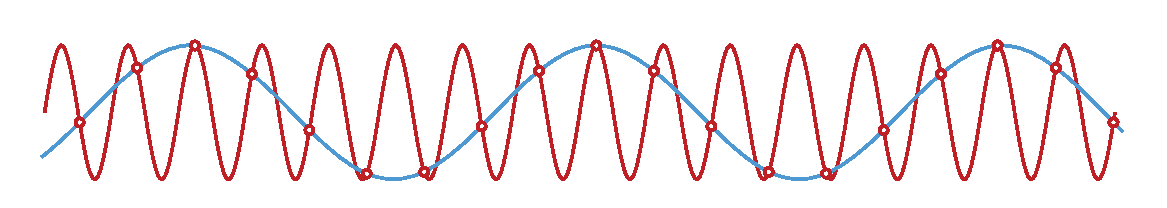
\includegraphics{antialias}}
\caption{\label{obr07} Ukážka aliasovania signálu}
\end{figure}

Na obrázku \ref{obr07} je názorná ukážka vzorkovania signálu s frekvenciou väčšou, ako je polovica vzorkovacej frekvencie. Tento signál sa do digitálnej podoby premietne ako signál s oveľa nižšou frekvenciou. Po takomto navzorkovaní sa už tento nežiaduci efekt vo všeobecnosti nedá odstraniť, takže jediný spôsob ako zabrániť aliasovaniu je odstrániť tieto vysoké frekvencie ešte pred vzorkovaním signálu.

Softvérový syntetizátor ale v žiadnej fáze generovania zvuku nepracuje s analógovým signálom, a preto je nutné nájsť spôsob, ako vytvárať tieto vlny antialiasované na všetkých počuteľných frekvenciách s celým počuteľným harmonickým spektrom.

Na vytvorenie vlny pre konkrétnu frekvenciu možno použiť Fouriérove rady. 

\subsubsection*{Píla}

\begin{equation*}
x(t) = \frac{2}{\pi} \sum_{k=1}^\infty \frac{\sin(2\pi k f t)}{k}
\end{equation*}

\subsubsection*{Obdĺžnik}

\begin{equation*}
x(t) = \frac{4}{\pi} \sum_{k=1}^\infty  \frac{\sin((2k-1) 2 \pi f t)}{(2k-1)}
\end{equation*}

\subsubsection*{Trojuholník}

\begin{equation*}
x(t) = \frac{8}{\pi^2} \sum_{k=1}^\infty \sin \left( \frac{k \pi}{2}\right) \frac{\sin(2\pi k f t)}{k^2}
\end{equation*}
\vspace{5mm}


Symbol $\infty$ pri generovaní je potrebné nahradiť konštantou $kmax$, pri ktorej by hodnota $kmax \times f$ bola menšia ako nyquistova frekvencia.

Tento spôsob síce vytvorí antialiasovanú vlnu pre konkrétnu frekvenciu, ale syntetizátor musí byť schopný vygenerovať akúkoľvek frekvenciu v rámci počuteľného spektra. Táto vlna by pri prehrávaní na vyššej frekvencii vytvárala aliasy a pri nízkej frekvencii by zas neobsahovala dostatok vysokých harmonických zložiek. 

Za najpraktickejšie riešenie tohto problému považujem vytvorenie tabuľky digitálnych vĺn s rôznym harmonickým obsahom pre každý priebeh. To znamená, že pre každý priebeh (píla, trojuholník, obdĺžnik) vytvorím tabuľku s určitým počtom vĺn rozmiestnených rovnomerne na logaritmickej frekvenčnej osi, napríklad jednu vlnu pre každú oktávu.

To by znamenalo, že každú vlnu budeme prehrávať maximálne v rozsahu jednej oktávy, čiže minimálna frekvencia prehrávania by bola polovica maximálnej. A teda, aby sme sa vyhli aliasovaniu, pri maximálnej frekvencii prehrávania vlny  pre vzorkovaciu frekvenciu 44\,100~Hz môže vlna obsahovať frekvencie do 22~kHz, ale prehrávaná na minimálnej frekvencii by jej najvyššia harmonická zložka mala len 11~kHz, a to by už bolo počuteľné orezanie vysokých frekvencií.

Ja som zvolil pre svoj syntetizátor odstupy jednotlivých digitálnych vĺn jednu tretinu oktávy, čiže 4 poltóny. Najnižšiu frekvenciu v tabuľke som zvolil 27,5~Hz, čo zodpovedá note A0, a harmonické zložky sa generujú po hranicu 20\,000~Hz. S odstupmi po 4 poltóny, až kým prvá harmonická zložka nie je nad hranicou 20\,000~Hz, je to spolu 27~vĺn. Vlny sa generujú v rozlíšení 384\,000~Hz, čo je dvojnásobok maximálnej komerčne používanej vzorkovacej frekvencie, aby sa zaručila čo najlepšia presnosť oscilátorov. 

Na generovanie akejkoľvek reálnej počuteľnej frekvencie sa budú vzorky prepočítavať z dvoch susedných vĺn lineárnou interpoláciou, pričom z každej vlny sa aktuálna vzorka počíta tiež lineárnou interpoláciou susedných hodnôt.

Výpočet frekvencie pre konkrétnu MIDI notu sa vykonáva vzorcom
\begin{equation*}
f = 440 \times 2^{\left(\frac{n-69}{12}\right)}
\end{equation*}
kde $n$ je číslo MIDI noty, $69$ je číslo noty A4, $440$ je frekvencia noty A4 v Hertzoch a $\frac{1}{12}$ je podiel noty v oktáve na logaritmickej osi.

\subsubsection{Parametre oscilátora}
\begin{description}
\setlength{\itemsep}{-0.5ex}
\item[Ladenie] -- Oscilátor musí mať možnosť pomerne presného ladenia vo veľkom rozsahu. V uživateľskom rozhraní to budú tri potenciometre: OCTAVE pre ladenie v rozsahu od --4 do +4 oktávy, COARSE po poltónoch vrozsahu od --12 do +12 poltónov, a FINE pre mikroladenie v rozsahu od --100 do +100 centov.
\item[Vlnový priebeh] -- Výber medzi spomínanými priebehmi.
\item[Synchronizácia] -- Možnosť synchronizovať s jedným iným oscilátorom metódou SoftSync\footnote{SoftSync -- pri tejto synchronizácii je fáza synchronizovaného oscilátora vynulovaná vždy, keď synchronizačný oscilátor začína novú periódu.}.
\end{description}

\subsection{Generátor obálky}

Obálka je veľmi dôležitý prvok pri syntéze, pretože definuje vývoj niektorého parametra, a tým aj celého zvuku v čase. Na obrázku \ref{obr08} sú načrtnuté parametre obálky a ich vplyv na jej priebeh.
\begin{figure}[h]
\centering
\resizebox{12cm}{!}{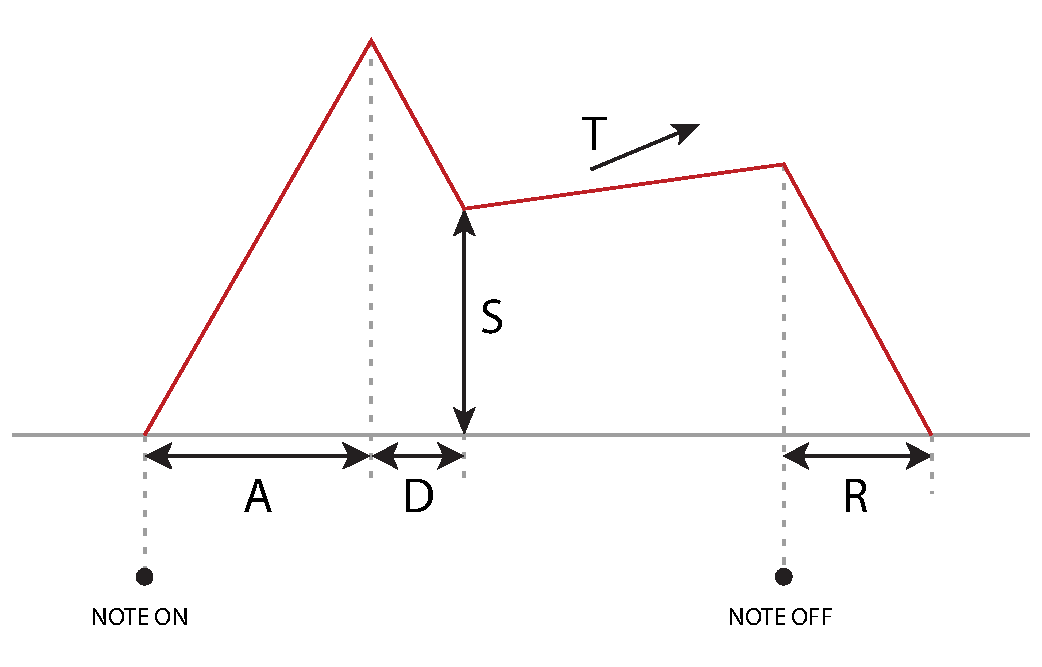
\includegraphics{adstr}}
\caption{\label{obr08} Obálka ADSTR}
\end{figure}

\subsubsection{Parametre obálky}
\begin{description}
\setlength{\itemsep}{-0.5ex}
\item[Attack] -- čas nábehu signálu na maximálnu hodnotu,
\item[Decay] -- čas poklesu signálu z maximálnej úrovne na úroveň SUSTAIN,
\item[Sustain] -- úroveň, na akú má signál klesnúť vo fáze DECAY s rozsahom 0 -- 100\,\%,
\item[Time] -- tendencia signálu stúpať alebo klesať po dosiahnutí hodnoty SUSTAIN, nadobúda hodnoty v rozsahu od --100\,\% do +100\,\%, kde 0\,\% znamená žiadne stúpanie/klesanie, kladné hodnoty určujú stúpanie a záporné klesanie.
\item[Release] -- čas poklesu úrovne signálu po uvoľnení klávesy na nulu.
\end{description}

Časové parametre majú rozsah 0 -- 12 sekúnd, pričom je potrebná väčšia hustota hodnôt blízko nuly ako pri vysokých hodnotách.

Obálka sa spúšťa prijatím MIDI udalosti NOTE ON. Po prechode fázami ATTACK a DECAY zotrváva vo fáze SUSTAIN až do prijatia správy NOTE OFF a prechádza do fázy RELEASE. V prípade prijatia správy NOTE OFF skôr, ako vo fáze SUSTAIN, sa rovnako prechádza do fázy RELEASE okamžite.

\subsection{LFO -- nízkofrekvenčný oscilátor}

Nízkofrekvenčný oscilátor využíva rovnaké priebehy ako oscilátor s dvoma rozdielmi:
\begin{itemize}
\setlength{\itemsep}{-0.5ex}
\item nízkofrekvenčný oscilátor nepotrebuje antialiasové opatrenia,
\item namiesto šumu využíva postupnosti náhodných hodnôt.
\end{itemize}

\subsubsection*{Priebeh náhodných hodnôt}

Syntetizátor využíva 2 typy priebehov náhodných hodnôt, pričom obidva generujú jednu náhodnú hodnotu pre každú periódu. Rozdiel medzi nimi je v tom, že prvý túto hodnotu drží počas celej periódy, pričom v druhom sa hodnoty susedných periód interpolujú.

\subsubsection{Parametre nízkofrekvenčného oscilátora}
\begin{description}
\setlength{\itemsep}{-0.5ex}
\item[frekvencia] -- frekvencia oscilátora v rozsahu 0,01~Hz -- 100~Hz,
\item[fázové posunutie] -- fázové posunutie oscilátora v rozsahu od --180° do +180°,
\item[opozdenie] -- čas opozdenia oscilácie v rozsahu 0 -- 12 sekúnd,
\item[nábeh] -- čas nábehu, čiže postupného zvyšovania amplitúdy oscilácie v rozsahu 0 -- 12 sekúnd,
\item[globálny/lokálny] -- prepínač, určujúci či bude oscilátor lokálny pre každý hlas alebo globálny pre všetky hlasy spolu.
\end{description}

Nízkofrekvenčný oscilátor je spúšťaný MIDI správou NOTE ON, spustí sa fáza opozdenia. Po uplynutí času opozdenia sa začína generovať signál s fázovým posunutím podľa hodnoty príslušného parametra. V čase nábehu sa amplitúda plynule zvyšuje z nuly na maximálnu úroveň.

\subsection{Filter}

Úloha filtra je odstrániť alebo potlačiť určité pásma frekvencií v signále. Pri analógových filtroch to robia RC články. V digitálnej doméne existujú dva druhy filtrov:

\begin{description}
\setlength{\itemsep}{-0.5ex}
\item[FIR] -- Finite Impulse Response -- filtre s konečnou dĺžkou impulzovej odozvy\footnote{Impulzová odozva je výstup zariadenia po poslaní impulzu na vstup. Impulz pre digitálne zariadenia je signál, kde prvá vzorka má maximálnu úroveň, a všetky nasledujúce majú hodnotu 0.}.
\item[IIR] -- Infinite Impulse Response -- filtre s nekonečnou dĺžkou impulzovej odozvy.
\end{description}

Digitálne filtre FIR fungujú na princípe spočítavania aktuálnych vzoriek s jednou alebo viacerými predchadzajúcimi vzorkami vynásobenými koeficientami filtra. Koeficienty filtra presne definujú frekvenčnú odozvu filtra\footnote{Frekvenčná odozva filtra opisuje vzťah medzi zložkami vstupného a výstupného signálu v závislosti od ich frekvencie.}. Rád filtra je maximum zo vzdialeností vzoriek použitých pri výpočtoch od aktuálnej vzorky. Ak filter využíva dve predošlé vzorky, je to filter druhého rádu.

Filtre IIR fungujú podobne ako filtre FIR, ale okrem predošlých vstupov používajú aj predošlé výstupy. Preto sa nazývajú aj filtrami so spätnou väzbou. Ich výhodou oproti filtrom FIR je, že dokážu pri nízkych rádoch poskytnúť strmé frekvenčné odozvy, na aké by bolo nutné použiť filter FIR oveľa vyššieho rádu. IIR filtre sú teda výpočtovo rýchlejšie, avšak nie je zaručená ich stabilita\footnote{Stabilita filtrov je tendencia impulzovej odozvy sa časom približovať k nule.} a tiež fázová odozva\footnote{Fázová odozva je vzťah fáz zložiek vstupného a výstupného signálu v závislosti od ich frekvencie.} sa pri nich ťažko udržiava lineárna.

Rád filtra je dôležitý parameter, pretože určuje strmosť filtrovania, a má tiež veľký vplyv na výpočtovú zložitosť filtrovania. V hudobných aplikáciách sa využívajú filtre so strmosťou 12 -- 24~dB na oktávu. Pre môj syntetizátor som zvolil IIR filter druhého rádu (označovaný aj ako \bq bikvadratický filter\eq \footnote{Bikvadratický filter -- tento názov je odvodený od prenosovej funkcie v Z-doméne, ktorá je definovaná ako pomer dvoch kvadratických funkcií.} , alebo \bq biquad\eq), ktorého schéma je na obrázku \ref{obr09}. Sériovým zapojením dvoch filtrov tohto typu vytvoríme filter so strmosťou 24~dB/oktávu.

\subsubsection*{Prenosová funkcia bikvadratického filtra}

\begin{equation*}
H(z) = \frac{b_0 + b_1\,z^{-1} + b_2\,z^{-2}}{1 + a_1\,z^{-1} + a_2\,z^{-2}}
\end{equation*}
Element $z^{-1}$ predstavuje opozdenie signálu o jednu vzorku, $b_0$, $b_1$, $b_2$, $a_1$ a $a_2$ sú koeficienty vypočítané z parametrov filtra.\newfootnote{Vzorce na výpočet koeficientov bikvadratického filtra sú opísané v dokumente \cite{b08}.}

\begin{figure}[h]
\centering
\resizebox{12cm}{!}{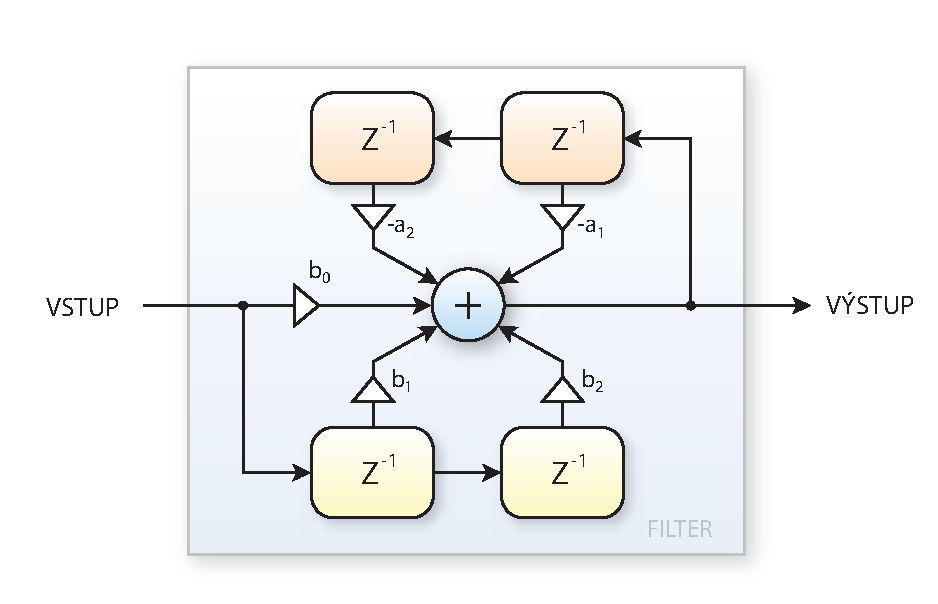
\includegraphics{filter}}
\caption{\label{obr09} Schéma bikvadratického filtra}
\end{figure}

\subsubsection{Parametre filtra}
\begin{description}
\setlength{\itemsep}{-0.5ex}
\item[Typ filtra] -- prepínač štyroch typov filtra (lowpass, highpass, bandpass, band-stop).
\item[Aktívna frekvencia] -- hraničná frekvencia pre typy lowpass a highpass, priepustná pre band-pass a filtrujúca pre band-stop. Rozsah týchto frekvencií je od 20~Hz do 20\,000~Hz.
\item[Q] -- rezonancia hraničného pásma pre typy lowpass a highpass, šírka pásma pre typy band-pass a band-stop. Rozsah parametra Q je 0 -- 10.
\item[Keyfollow] -- miera vplyvu výšky zahratej noty na aktívnu frekvenciu v rozsahu od --100\,\% do +100\,\% (0\,\% - žiadny vplyv, +100\,\% - aktívna frekvencia sa posúva presne podľa frekvencie zahratej noty, --100\,\% - aktívna frekvencia sa posúva v rovnakých intervaloch, ako zahratá nota, ale v opačnom smere).
\item[Mix] -- percentuálny podiel signálu, ktorý je filtrovaný.
\end{description}

\subsection{Mixér}

Mixér je komponent, ktorý sčítava signály z oscilátorov.

\subsubsection{Parametre mixéra}
\begin{description}
\setlength{\itemsep}{-0.5ex}
\item[Úroveň oscilátorov] -- percentuálna úroveň signálu pre každý oscilátor.
\item[Smerovanie oscilátorov] -- smerovanie signálu pre každý oscilátor. Hodnoty parametra sú v rozsahu 100L -- 0 -- 100R. Hodnoty predstavujú percentuálne umiestnenie signálu od stredu doľava (L) alebo doprava (R).
\end{description}

\subsection{Zosilňovač}

Zosilňovač je komponent, ktorý umožňuje regulovať úroveň signálu z mixéra. Jeho úloha v digitálnych syntetizátoroch nie je taká podstatná. V navrhovanom syntetizátore sprostredkúva moduláciám celkovú úroveň hlasu. Tento komponent nemá žiadne ovládacie parametre.

\subsection{Modulačná matica}

Modulačná matica obsahuje 32 slotov pre aplikáciu modulácií.

\subsubsection{Parametre modulačných slotov}
\begin{description}
\setlength{\itemsep}{-0.5ex}
\item[Zdroj modulácie] - predstavuje modulačný signál.
\item[Cieľ modulácie] - predstavuje modulovaný parameter.
\item[Miera modulácie] - miera modulácie v percentách v rozsahu od --100\,\% do +100\,\%. Záporné hodnoty vynásobia modulačný signál hodnotou --1.
\end{description}

\noindent
Zdrojom modulácie môže byť:
\begin{itemize}
\setlength{\itemsep}{-0.5ex}
\item MIDI správa,
\item obálka,
\item signál z nízkofrekvenčného oscilátora.
\end{itemize}

Cieľom modulácie môže byť každý spojitý parameter syntetizátora okrem miery modulácie.

Modulačný signál sa pri modulácii pripočítava k hodnote parametra vynásobený mierou modulácie. Výnimkou je modulácia úrovní signálov oscilátorov mixéra alebo celkovej úrovne zosilňovača obálkami alebo MIDI správami CC. Vo vymenovaných prípadoch dochádza k násobeniu namiesto sčítavania a pri zápornej miere modulácie obálkami sa signál obálok posúva pripočítaním maximálnej úrovne signálu obálok do nezáporných hodnôt. 

\subsection{Interpolácia hodnôt parametrov}

Nespojitá zmena spojitých parametrov môže v mnohých prípadoch spôsobiť nežiaduce efekty vo zvukovom výstupe. Preto je potrebné takto citlivé parametre ošetriť pred nespojitou zmenou interpoláciou novej hodnoty s hodnotou pôvodnou. Na tento účel plne postačuje lineárna interpolácia s pevným časom prechodu z pôvodnej hodnoty do novej. Pre tento čas som určil hodnotu 50 milisekúnd.

\section{Perzistentné ukladanie nastavení}

Pre prácu so syntetizátorom je nevyhnutná možnosť uloženia aktuálnych nastavení parametrov a ich obnovenia kedykoľvek podľa potreby. Tiež je dôležité, aby sa tieto nastavenia ukladali automaticky pri ukladaní projektu hostiteľskej aplikácie a aby sa obnovili spolu s obnovením projektu. 

Zoznam nastavení parametrov syntetizátora je v terminológii VST \textbf{program}. Často sa v rovnakom význame používajú aj termíny \emph{preset} a \emph{patch}. Množina viacerých programov sa označuje termínom \textbf{banka}.

VST SDK vo verzii 2.4 ponúka možnosť uložiť aktuálne nastavenia hostiteľským programom bez nutnosti implementácie takejto funkcionality v syntetizátore. Tento automatický spôsob ukladania nastavení hostom má niekoľko výhod:

\begin{itemize}
\setlength{\itemsep}{-0.5ex}
\item programátor nemusí implementovať metódu pre ukladanie nastavení,
\item o ukladanie nastavení sa stará host, ktorý by mal zaručiť platformovo nezávislý spôsob uloženia,
\item host má väčšie možnosti manipulácie s nastaveniami.
\end{itemize}

Z týchto dôvodov som sa rozhodol využiť tento spôsob perzistentného uloženia programov.

\section{Návrh GUI}

Pre grafické používateľské rozhranie som si stanovil nasledovné požiadavky:

\begin{description}
\setlength{\itemsep}{-0.5ex}
\item[Prehľadnosť] -- na prvý pohľad musí byť jasné, ktorá časť grafického rozhrania na čo slúži. Komponenty by mali byť veľmi rýchlo rozoznateľné, zreteľne označené názvom. Ovládacie prvky musia byť rozoznateľné od statických grafických prvkov. Vlnové priebehy, obálky a filtre môžu byť pre väčšiu prehľadnosť graficky interpretované.
\item[Estetickosť] -- návrh musí rešpektovať pravidlá estetickosti, využívať harmonické farby a pôsobiť príjemne.
\item[Jednoznačnosť] -- podoba komponentov, ich rozmiestnenie a označenie musia jednoznačne identifikovať ich funkciu.
\item[Ovládateľnosť] -- parametre musia byť jednoducho ovládateľné, musí byť viditeľná ich aktuálna hodnota. 
\end{description}

Pre návrh som zvolil ako základnú farbu bledomodrú a použil rôzne farby pre rôzne komponenty. Spojité parametre sú navrhnuté na spôsob potenciometrov. Každý je zreteľne označený a každý má zobrazenú aktuálnu hodnotu na príslušnom displeji pod potenciometrom. Nespojité parametre sú interpretované formou grafických alebo textových tlačidiel. Priebehy oscilátorov, nízkofrekvenčných oscilátorov, frekvenčné odozvy filtrov sú názorne zobrazené na tlačidlách zmeny týchto parametrov. Tvar obálky sa vykresľuje na displeji v reálnom čase zmenou parametrov. Modulačná tabuľka používa na výber zdrojov a cieľov vyrolovacie menu. Návrh je zobrazený na obrázku \ref{obr10}.

\begin{figure}[h]
\centering
\resizebox{14cm}{!}{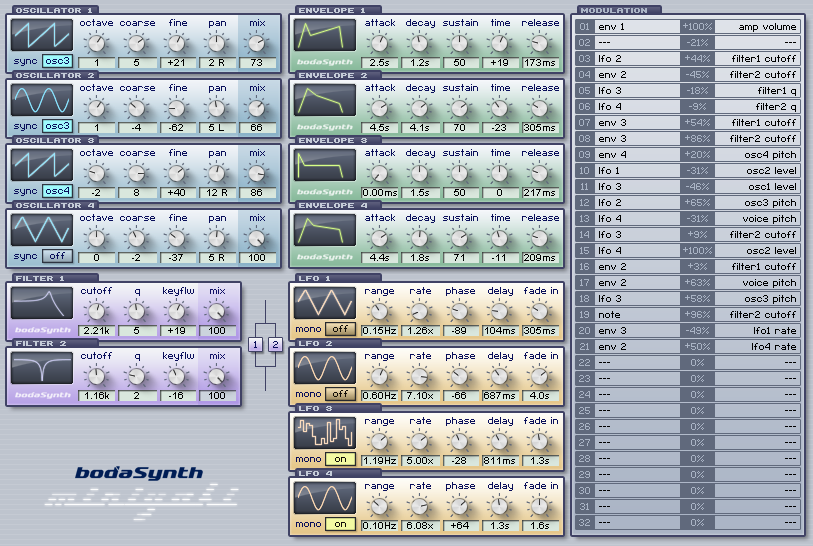
\includegraphics{gui}}
\caption{\label{obr10} Návrh GUI}
\end{figure}
